\documentclass[12pt,a4paper]{article}

\usepackage[utf8]{inputenc}
\usepackage[T1]{fontenc}
\usepackage[english]{babel}
\usepackage{graphicx}
\usepackage{float}
\usepackage{hyperref}
\usepackage{geometry}
\geometry{margin=2.5cm}

\title{Prognostic Module --- User Guide\\[0.5em]
\large Czech Salivary Gland Database}
\author{}
\date{}

\begin{document}

\maketitle
\tableofcontents
\newpage

\section{Prognostic Module -- User Guide}\label{app:prognosticModuleUserGuide}
The prognostic module allows users to calculate risk predictions for individual patients using trained machine learning models, retrain models on the current database, and inspect information about all available models.

The complete Czech version of the manual is available in the \texttt{README.md} file on GitHub\footnote{\url{https://github.com/vjelinekk/CzechSalivaryGlandDB}}.

\subsection{Calculating a Prediction}
\begin{enumerate}
    \item Navigate to the \textit{Patient List} section.
    \item Select the patient for whom you want to calculate a prognostic score.
    \item Click the head-with-gear icon in the upper right corner (Figure~\ref{fig:pred-calc-1}).

    \begin{figure}[H]
        \centering
        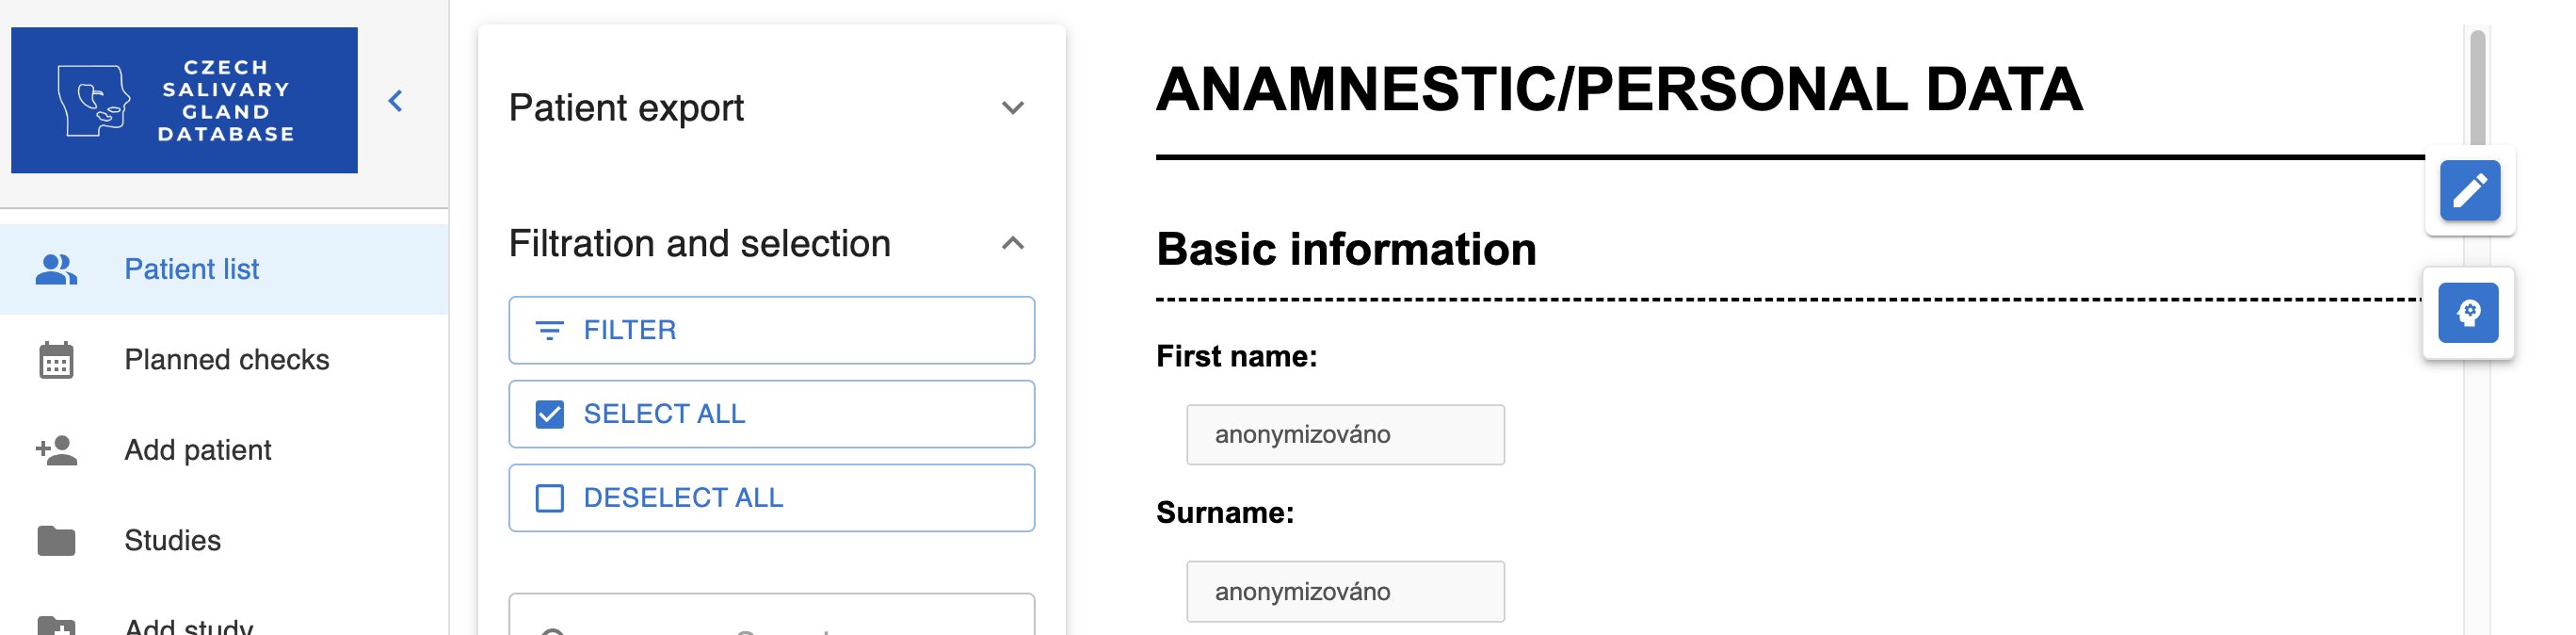
\includegraphics[width=0.8\textwidth]{img/prediction_calculation_1.png}
        \caption{Opening the prognostic module for a patient.}
        \label{fig:pred-calc-1}
    \end{figure}

    \item Select the type of prediction you want to calculate (Figure~\ref{fig:pred-calc-2}).

    \begin{figure}[H]
        \centering
        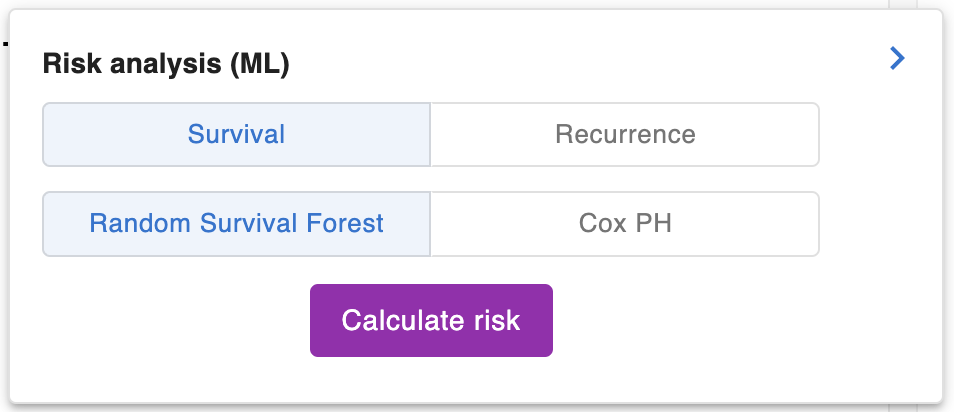
\includegraphics[width=0.8\textwidth]{img/prediction_calculation_2.png}
        \caption{Selecting the prediction type.}
        \label{fig:pred-calc-2}
    \end{figure}

    \item Click the \textit{Calculate risk} button.
    \item The calculation will run and the result will be displayed (Figure~\ref{fig:pred-calc-3}).

    \begin{figure}[H]
        \centering
        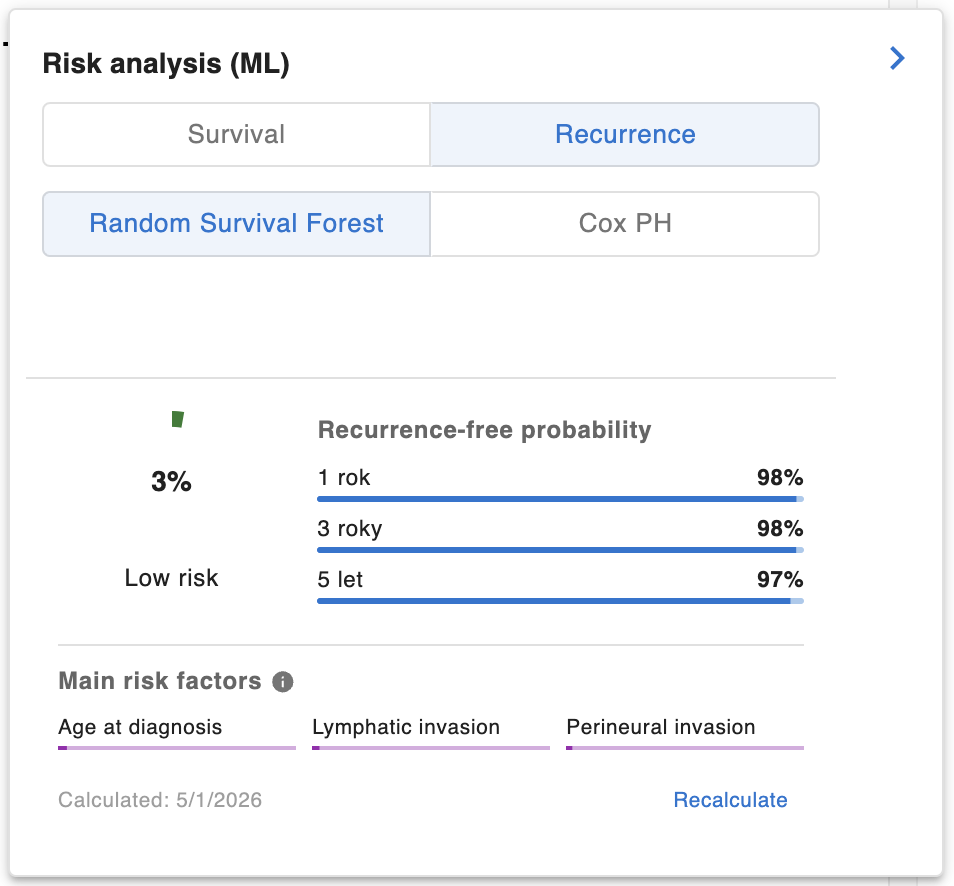
\includegraphics[width=0.8\textwidth]{img/prediction_calculation_3.png}
        \caption{Prediction result.}
        \label{fig:pred-calc-3}
    \end{figure}
\end{enumerate}

\subsection{Training a Model}

\begin{enumerate}
    \item Navigate to the \textit{Risk Prediction (ML)} section.
    \item Select which model you want to train (Figure~\ref{fig:pred-train-1}).

    \begin{figure}[H]
        \centering
        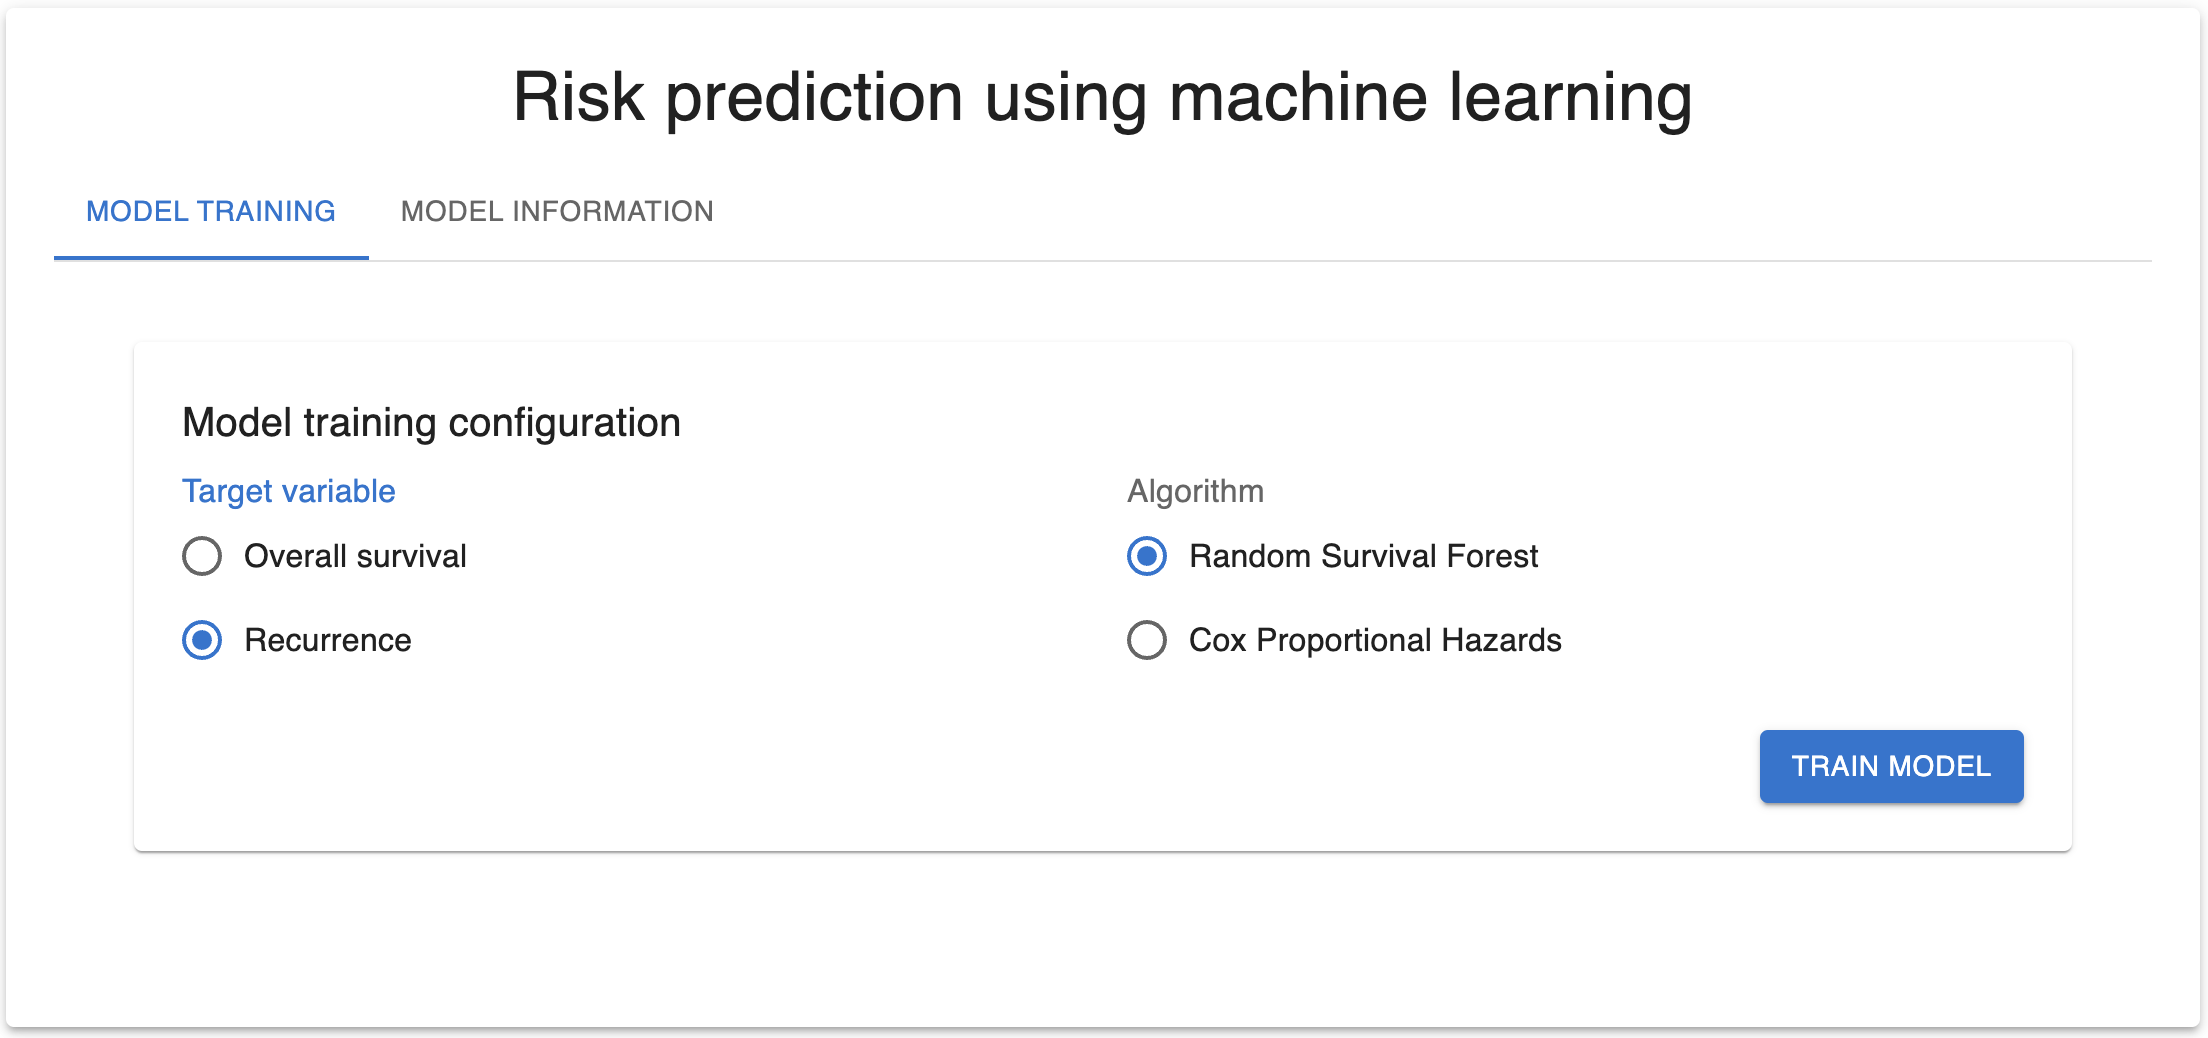
\includegraphics[width=0.8\textwidth]{img/prediction_training_1.png}
        \caption{Selecting a model for training.}
        \label{fig:pred-train-1}
    \end{figure}

    \item Start the training by clicking the \textit{TRAIN MODEL} button.
    \item Once training is complete, the training result is displayed (Figure~\ref{fig:pred-train-2}).

    \begin{figure}[H]
        \centering
        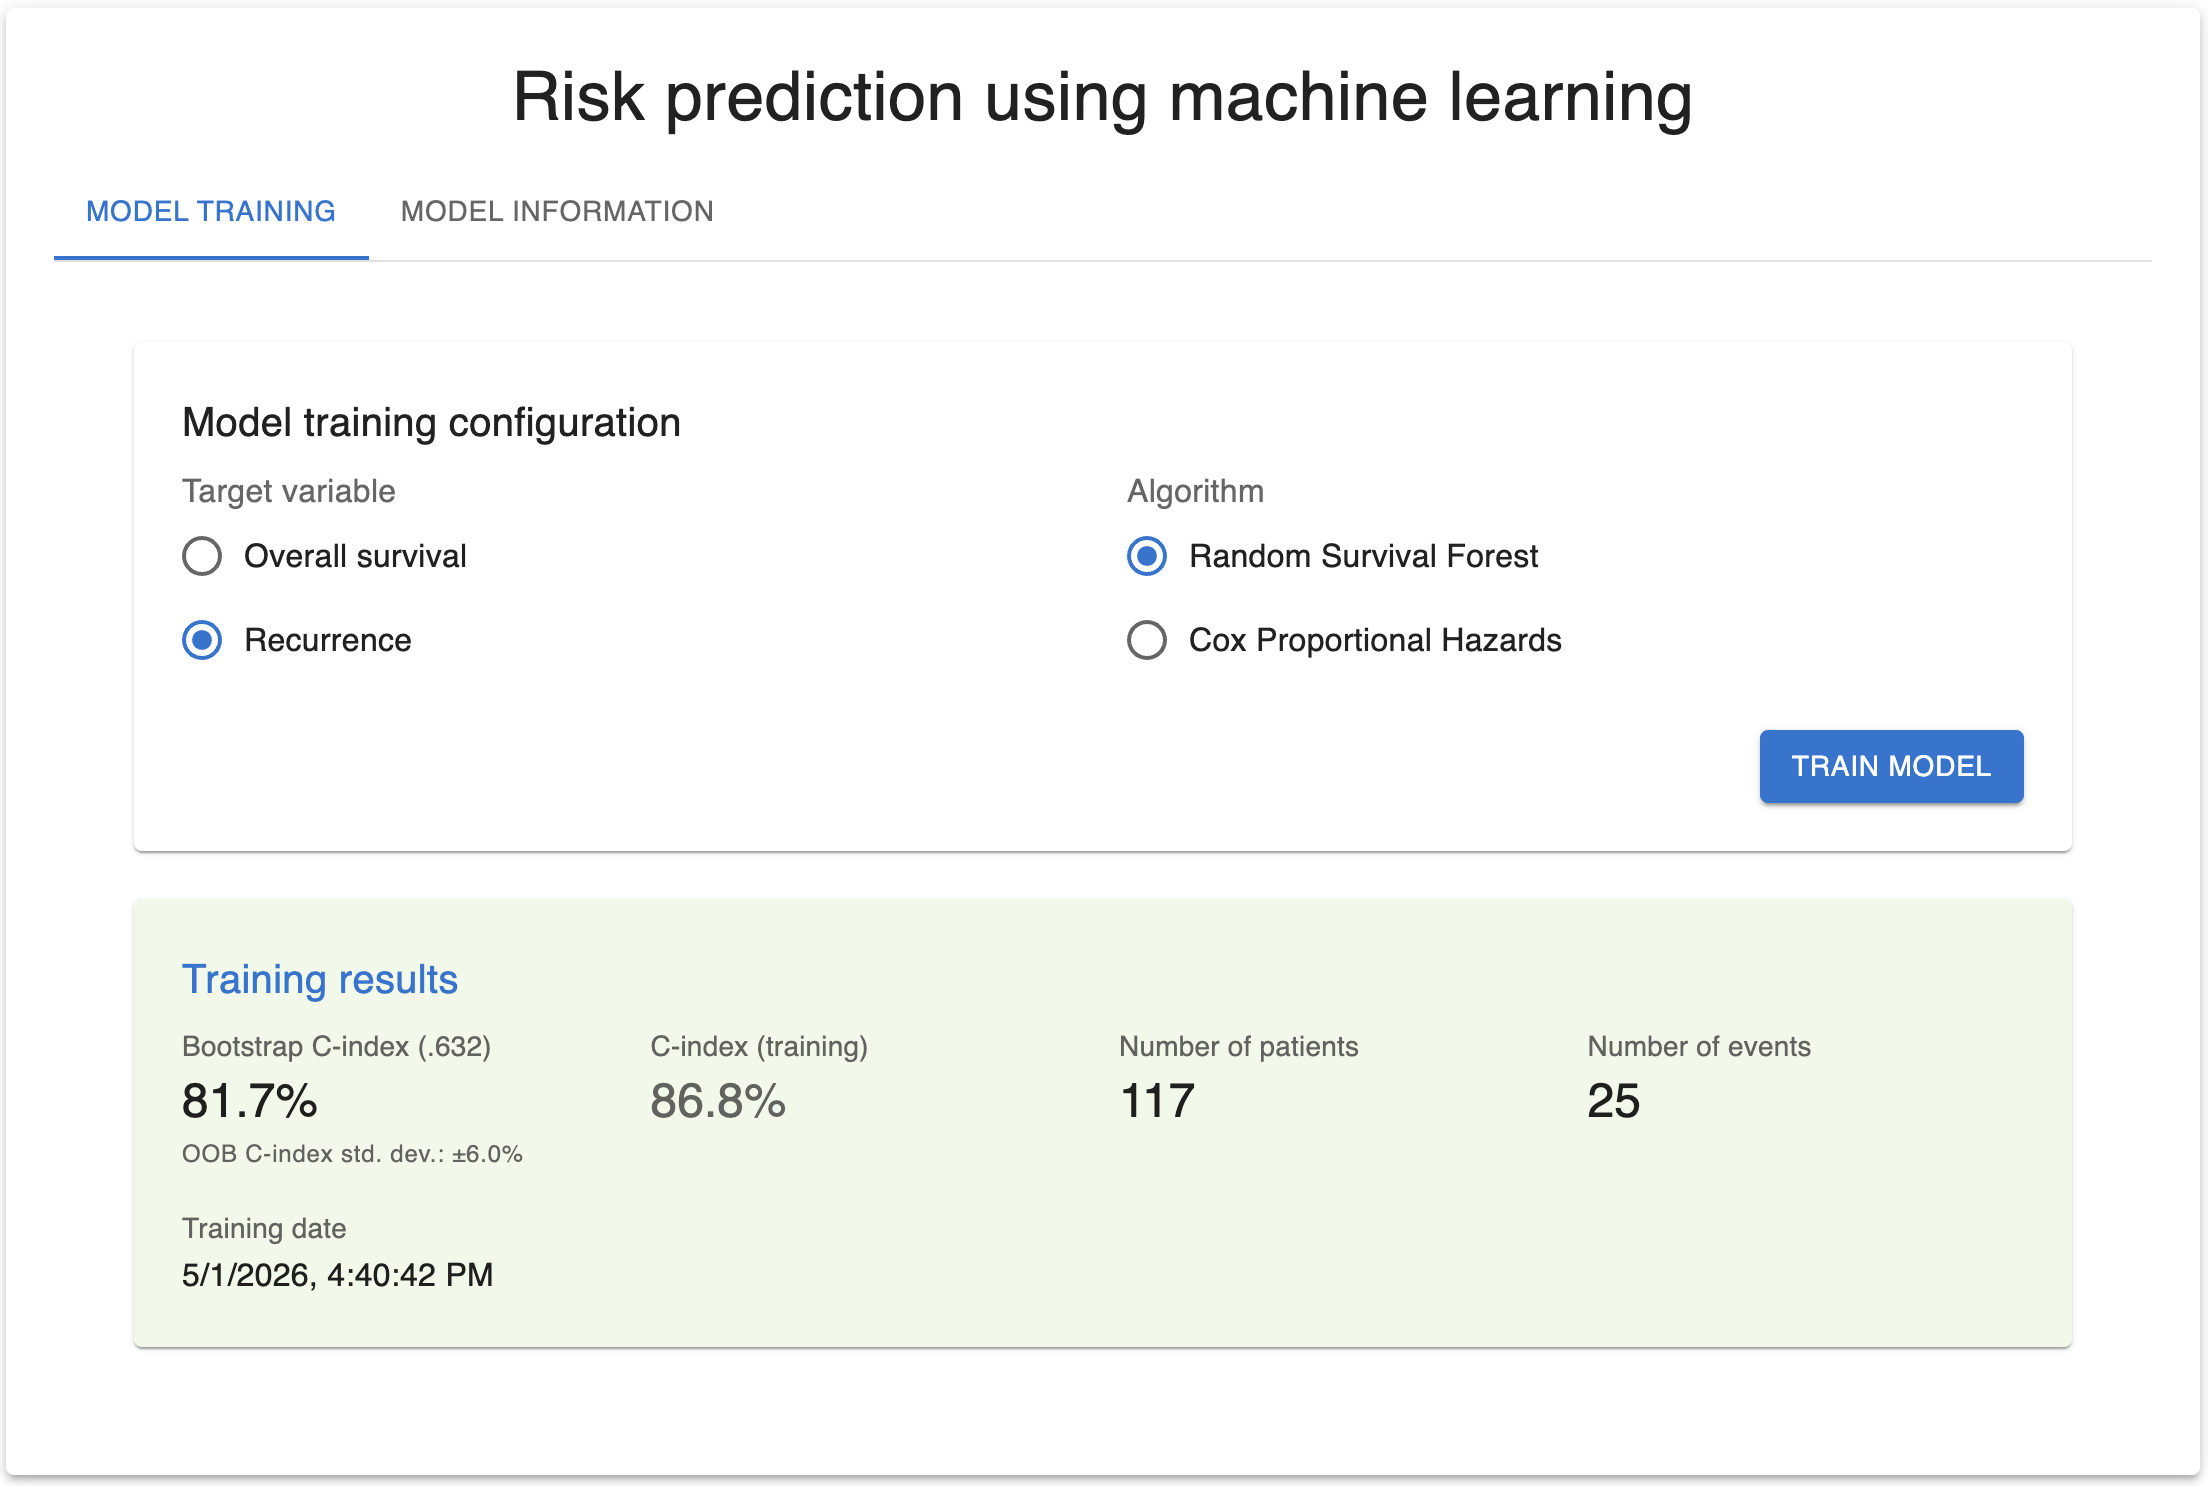
\includegraphics[width=0.8\textwidth]{img/prediction_training_2.png}
        \caption{Training result after completion.}
        \label{fig:pred-train-2}
    \end{figure}
\end{enumerate}

\subsection{Model Information}

\begin{enumerate}
    \item Navigate to the \textit{Risk Prediction (ML)} section.
    \item Switch to the \textit{Model Information} tab (Figure~\ref{fig:pred-info}).

    \begin{figure}[H]
        \centering
        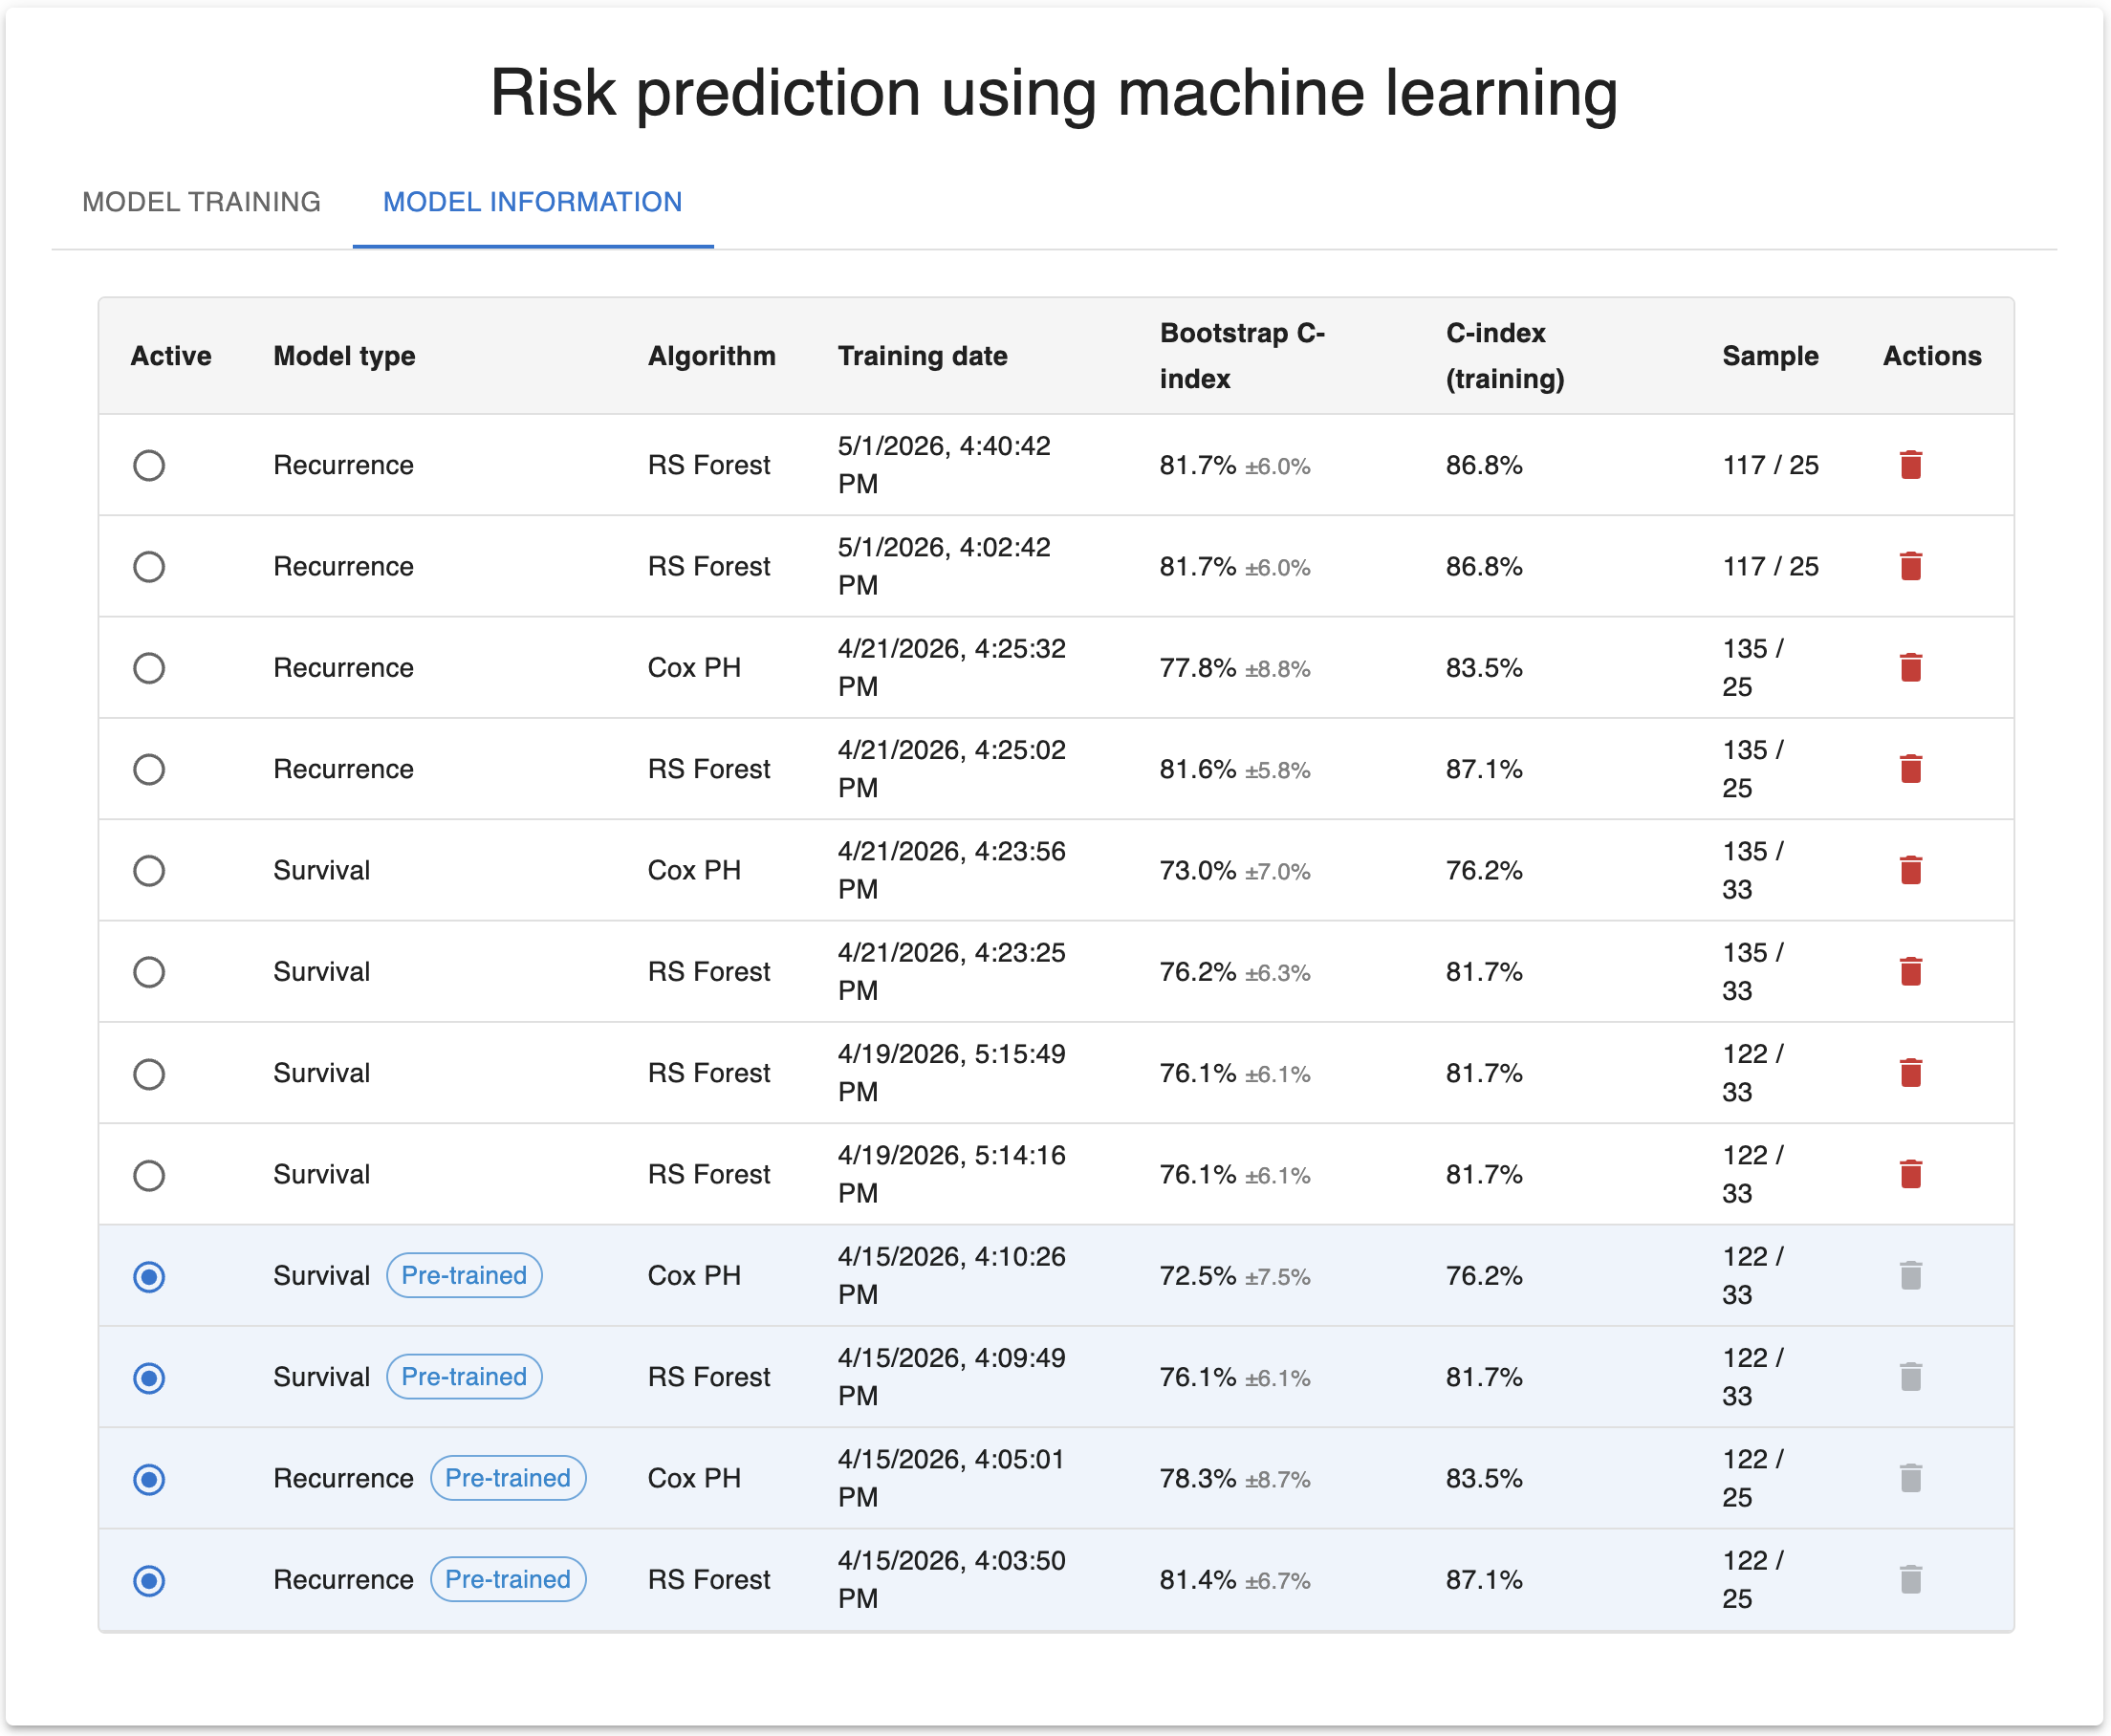
\includegraphics[width=0.8\textwidth]{img/prediction_info.png}
        \caption{Model information tab showing all trained and active models.}
        \label{fig:pred-info}
    \end{figure}

    \item A list of all trained and currently active models is shown here.
    \item You can select the active model and also delete not active models.
\end{enumerate}

\end{document}